\documentclass[aspectratio=169]{beamer}
\setbeamertemplate{navigation symbols}{}
\usepackage{color,amsmath,comment, subfigure}
\usepackage{booktabs}
\usepackage{url}

%\setbeameroption{show notes}

%%%%%%%%%%%%%%%%%%%%%%%%%%
\title[]{Class 9: Madness of crowds}
\author[]{Matthew J. Salganik}
\institute[]{Sociology 204: Social Networks\\Princeton University}
\date[]{
2/2 Consequences of interdependent individual decisions: Information cascades

\vfill 

\begin{flushleft}
\vspace{0.6in}
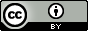
\includegraphics[width=0.1\textwidth]{figures/cc.png}
\end{flushleft}

}

\note{

possibly move the candy bowl to previous class so that they do it without benefit of readings

% TODO: add The Sound of Silence: Observational Learning in the U.S. Kidney Market https://pubsonline.informs.org/doi/10.1287/mksc.1090.0500
% TODO: add 4 criteria from Easley Kleinberg Sec 16.2
}

\begin{document}
%%%%%%%%%%%%%%%%%%%%%%%%%%%
\frame{\titlepage}
%%%%%%%%%%%%%%%%%%%%%%%%%%%
\begin{frame}

What happens if we have a bunch of people who are all being influenced by each other?

\note{
Information cascade
}

\end{frame}
%%%%%%%%%%%%%%%%%%%%%%%%%
\begin{frame}

{\small 

\begin{table}
\center
\begin{tabular}{cccccc}
\toprule
                         & \onslide<1->{Alice} & \onslide<4->{Bob} & \onslide<6->{Clarence} & \onslide<8->{David} & \onslide<10->{Edgar} \\
\midrule
Private Signal & \only<2,3>{shot bad} \only<4->{\textcolor{lightgray}{shot bad}} & \only<4,5>{shot bad} \only<6->{\textcolor{lightgray}{shot bad}} & \only<6,7>{shot good} \only<8->{\textcolor{lightgray}{shot good}} & \only<8,9>{shot good} \only<10->{\textcolor{lightgray}{shot good}} & \only<10,11>{shot good} \only<12->{\textcolor{lightgray}{shot good}}  \\
Public Action & \onslide<3->{no shot} & \onslide<5->{no shot} & \onslide<7->{no shot} & \onslide<9->{no shot} & \onslide<11->{no shot} \\
\bottomrule
\end{tabular}
\end{table}

}

\note{

Let's consider a discrete case.  Consider the decision of whether or not to get a flu shot (is this something you have to decide?.  Let's also assume that the flu shot is really good for everyone (I am not a real doctor so this might not be a good assumption).  Now, each person gets a private signal ``flu shot good'' with probability $p > 0.5$ and ``flu shot bad'' with probability $1-p$.  Now image that Alice gets signal ``flu shot bad'' and she don't get the flu shot.  Then Bob also get signal ``flu shot bad.'' Bob sees that Alice did not get it either so he don't get it.  Now Clarence comes along, and gets the signal ``flu shot good'', but he also see that the previous two people  (Bob and Alice) did not get the shot.  Given the model of decision making they propose, Clarence will not get the flu shot because he guesses that there were two negative signal and one possible signal.  Now imagine that David, Edgar, Francine, etc. all get ``flu shot good'' none of them will adopt because they assume all the previous people got ``flu shot bad''.

When we make a decision we often have two pieces of information ``private signal'' and ``behavior of others''.  Think about the sequential candy guessing.  Note that ``behavior of others'' is not ``private signal'' of others.  For example, in candy guessing people might have changed their stated answer based on the behavior of others.

Model in Easley and Kleinberg is nice because you can see how they build it up.  Just in case you wonder those technical details will not be on necessary for the midterm, but for your life outside of Princeton the ability to take a complicated problem and break it down to its essence will be very important.  The process that Easily and Kleinberg go through in this chapter is an important model of that.

Once a cascades starts information stops accumulating because we only see public behavior not private signal and at a certain point private signal can be overwhelmed by public information.  People are following people who are following people, who are following people. . . 
}

\end{frame}
%%%%%%%%%%%%%%%%%%%%%%%%%%
\begin{frame}

This example highlights some important points about information cascades:
\begin{enumerate}
\item cascades can occur pretty easily 
\pause
\item cascades can lead to non-optimal outcomes
\pause
\item can be fragile (if someone is willing to break them)
\pause
\item cascades depend on the difference between private signal and public behavior
\end{enumerate}

\end{frame}
%%%%%%%%%%%%%%%%%%%%%%%%%%
\begin{frame}

Could something like this really happen?

\begin{figure}
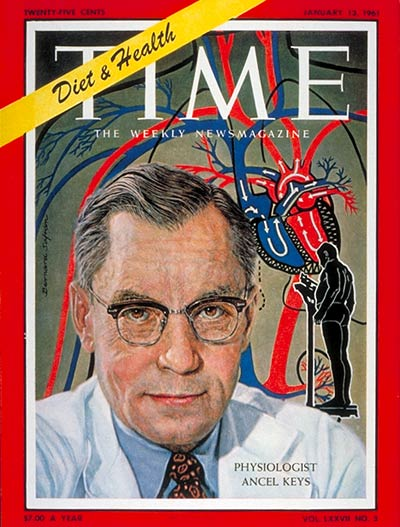
\includegraphics[height=0.70\textheight]{figures/ancel_keys_time}
\end{figure}


\end{frame}
%%%%%%%%%%%%%%%%%%%%%%%%%%
%\begin{frame}
%
%Candy results
%
%\note{
%s
%This is the wisdom of crowd that is often though to apply to markets.  The second situation is more like the world than the first.  Interdependent behavior is more common and more complex.  It depends on all kinds of things, like who speaks first, the size of the class, how well you know each other, etc.  In the next three lectures we are going to learn about interdependence and what it means for collective dynamics.\\
%}
%
%\end{frame}
%%%%%%%%%%%%%%%%%%%%%%%%%%
\begin{frame}

Summary:
\begin{itemize}
\item many decisions are interdependent
\pause
\item when there are interdependent decisions, individual rationality can lead to collective irrationality
\end{itemize}

\end{frame}
%%%%%%%%%%%%%%%%%%%%%%%%%%
\begin{frame}

Next class:
\begin{itemize}
\item Gladwell, M. (1996). The tipping point. \textit{The New Yorker}. 
\item Watts, Chapter 8.
\item Watts, D.J. (2002). A simple model of global cascades on random networks. \textit{Proceedings of the National Academy of Sciences}. (Warning: this paper has hard math)
\end{itemize}

\end{frame}
%%%%%%%%%%%%%%%%%%%%%%%%%%

\end{document}
